\documentclass[10pt]{beamer}
\usepackage{amsmath} % For math symbols
\usepackage{centernot}
\usepackage{graphicx}
\usetheme{metropolis}
\usepackage{appendixnumberbeamer}

\usepackage{booktabs}

\usepackage{pgfplots}
\usepgfplotslibrary{dateplot}

\usepackage{xspace}
\newcommand{\themename}{\textbf{\textsc{metropolis}}\xspace}

\title{Deep Residual Learning for Image Recognition}
\subtitle{A Review}
\date{March 10, 2020}
\author{Abhishek Ranjan}
\institute{Toronto, ON}
% \titlegraphic{\hfill\includegraphics[height=1.5cm]{logo.pdf}}

\begin{document}

\maketitle

\begin{frame}{Table of contents}
  \setbeamertemplate{section in toc}[sections numbered]
  \tableofcontents [hideallsubsections]
\end{frame}

\section{The Problem}
%--------------------------
	\begin{frame}[fragile]{Difficulties in Deep NN Training}
		\begin{enumerate}
			\item Vanishing/exploding gradients; claimed to be addressed by:
			\begin{itemize}
				\item Batch Normalization in forward propagation
				\item ReLU + weight initialization
			\end{itemize}
			\item Degradation problem (Figure \ref{fig-degradation}):
				\begin{figure}
					\centering
					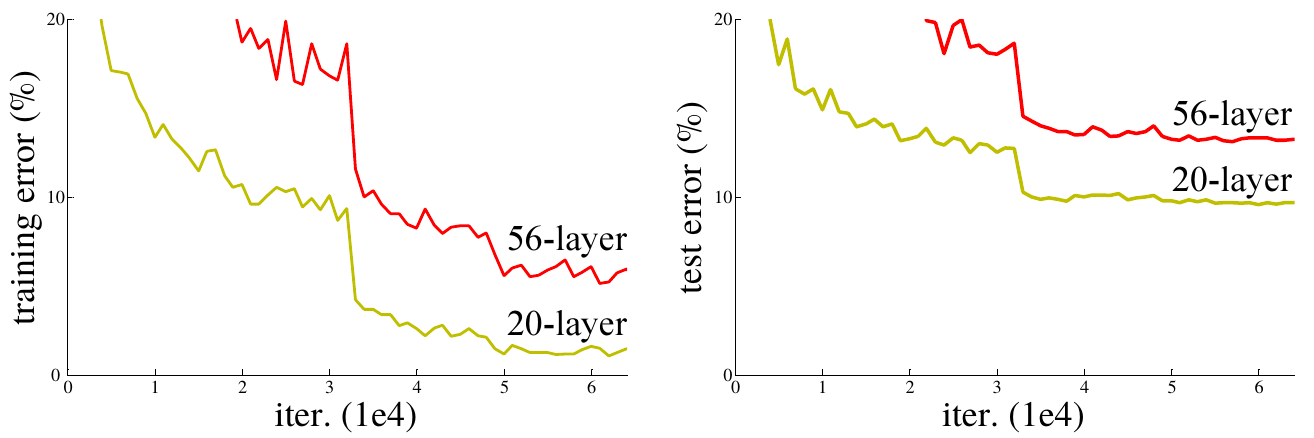
\includegraphics[width=0.8\textwidth]{degradation-problem.png}
					\caption{Degradation problem for CIFAR-10}
					\label{fig-degradation}
				\end{figure}
		\end{enumerate}
	\end{frame}

	\begin{frame}[fragile]{Degradation problem}
		Degradation problem posed as originating from the solver 
		\begin{itemize}
			\item Increasing depth $\centernot\implies$ Low error
			\item Training error is also high $\implies$ Not an overfitting problem
			\item Possible causes: difficulty in learning Identity functions
		\end{itemize}
	Problem statement: \textbf{Can we increase depth without degrading accuracy?} \cite{resnet_he2016}
	\end{frame}

\section{Fundamental Ideas}

	\begin{frame}[fragile]{Proposed solution}
		Make it easy for the solver to reach identity mapping		
		\begin{itemize}
			\item Force identity shortcuts for $x$ to reach the output
			\item If the original block learns $H(x)$, after shortcut it learns $F(x) = H(x) - x$
		\end{itemize}
		Why residuals?
		\begin{itemize}
			\item Residuals are easier to learn (evidenced by other areas)
			\item Solver can move the weights to zero more easily than to identity mapping
			\item No extra parameters (for most cases)
		\end{itemize}
		\small{\textit{Note: No mathematical justification provided in the paper, mostly empirical.}}
	\end{frame}

	\begin{frame}[fragile]{Architecture example}
		\begin{enumerate}
			\item Start with a deep, plain network, e.g., a VGG n/w with 34 layers (3x3 Convolutional filters)		
			\item Add shortcut connections (Figure \ref{fig-shortcut})
				\begin{itemize}
					\item Identity connections every 2 blocks when dimensions match
						\begin{figure}
						\centering
						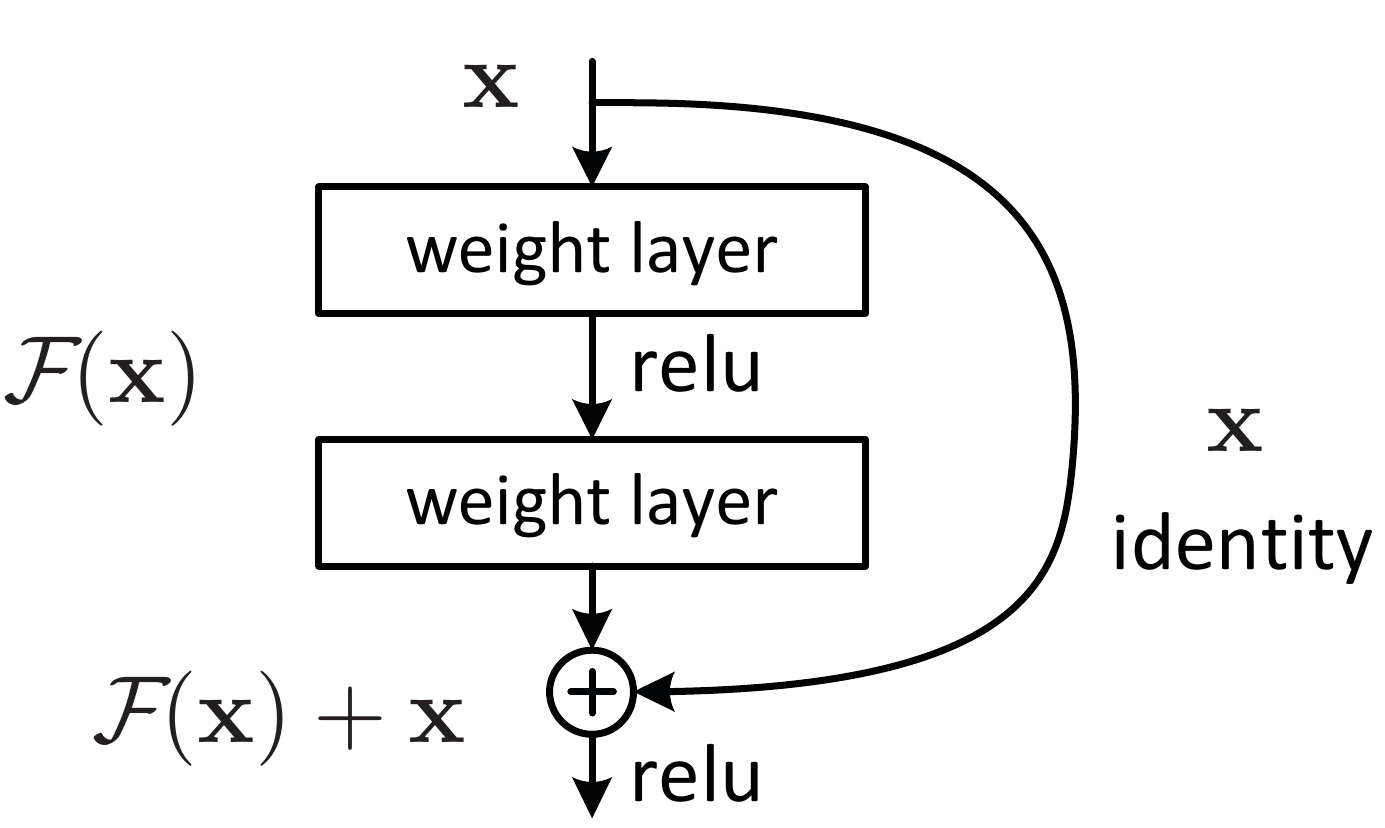
\includegraphics[width=0.4\textwidth]{residual_conn}
						\caption{Identity shortcut example}
						\label{fig-shortcut}
						\end{figure}
					\item When dimensions don't match:
						\begin{enumerate}
							\item Use identity mapping with zero-padding (no extra params)
							\item Use projection shortcut (more params!)
						\end{enumerate}
				\end{itemize}
			\end{enumerate}
	\end{frame}

	\begin{frame}{Training}
		\begin{itemize}
			\item Train as usual with SGD + backpropagation
			\item Batch normalization after convolution before ReLU
			\item Learn rate $\eta=0.1$, weight decay $\lambda = 0.0001$, momentum $\alpha=0.9$
			\item Weight initialization \cite{delving_deeper_he2015}: $N(0, \sigma=\sqrt(2/fan_{in}))$
			\item For bottleneck architecture: use identity shortcuts to avoid complexity 
		\end{itemize}
	\end{frame}

\section{Results and Conclusions}
	\begin{frame}{Accuracy}
		Significant improvements in training and validation error across the board
		\begin{figure}
			\centering
			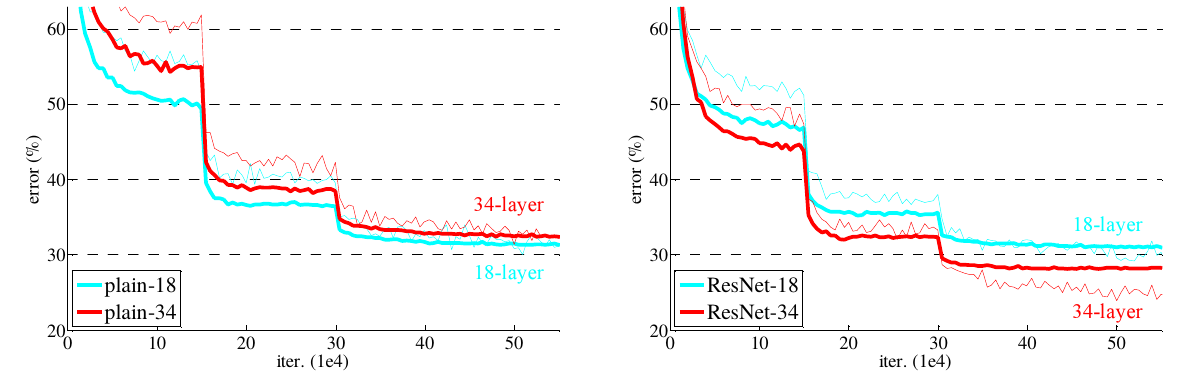
\includegraphics[width=\textwidth]{results-imagenet-1.png}
			\caption{Training (bold line) and validation (thin line) error on ImageNet}
			\label{fig_results_imagenet}
		\end{figure}
	\end{frame}

	\begin{frame}{Layer responses}
		ResNet layer responses are smaller $\implies$ Identity shortcuts pass most information 
		\begin{figure}
			\centering
			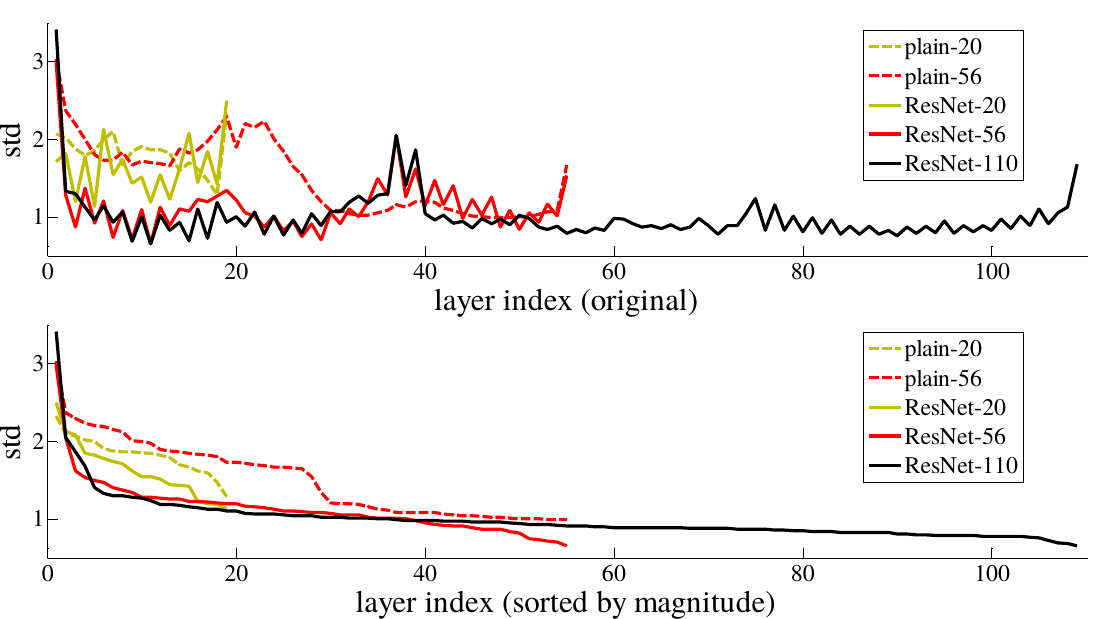
\includegraphics[width=\textwidth]{layer-response.png}
			\caption{Standard deviation of layer responses on CIFAR-10}
			\label{fig_layer_response}
		\end{figure}		
	\end{frame}

	\begin{frame}{Conclusions}
		\begin{itemize}
			\item Proposed a new architecture using residuals to address degradation problem
			\item Identity shortcuts mostly add no extra parameters
			\item Significant increase in number of layers possible
			\item Provided strong empirical evidence of its effectiveness across a wide range of tasks
			\item Opens up many research areas and raises questions:
				\begin{itemize}
					\item What is the nature of the degradation problem?
					\item Is the degradation problem really separate from unstable gradients problem?
					\item How do shortcut connections allow deeper networks (mathematically)?
				\end{itemize}  
		\end{itemize}
	\end{frame}

	\begin{frame}[standout]
		Questions and Discussion
	\end{frame}

%===================================================
\appendix

\begin{frame}{An ensemble of shallow networks \cite{resnet_as_ensemble_shallow_veit2016}}
	\begin{itemize}
		\item A collection of many paths of different length (Figure \ref{fig_multi_path})
		\item Avoids vanishing gradients by leveraging only the short paths
		\item Layers behave like ensembles
	\end{itemize}
	\begin{figure}
		\centering
		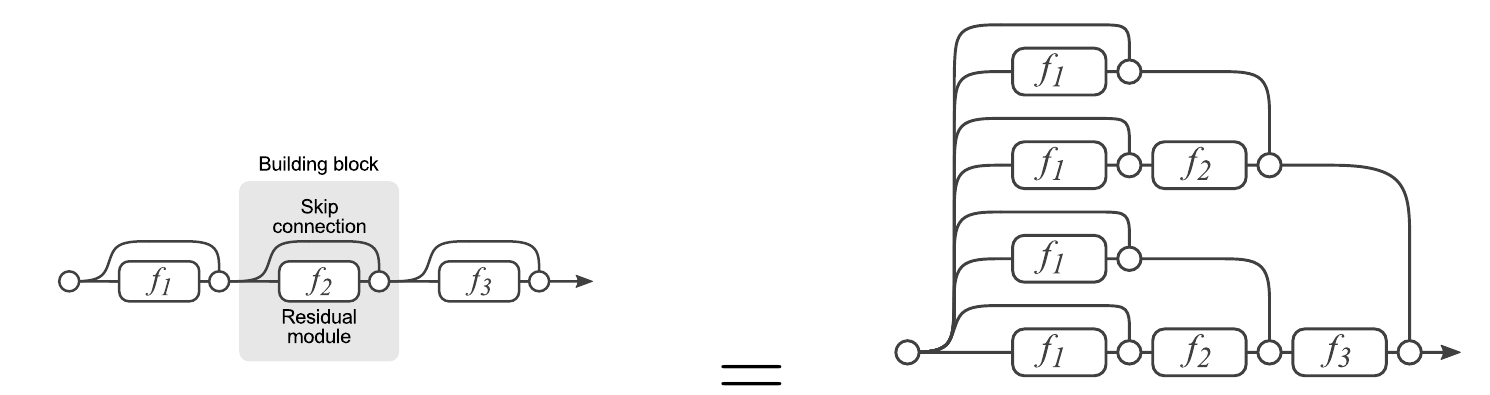
\includegraphics[width=\textwidth]{resnet_as_multiple_paths.png}
		\caption{Unraveled paths of residual connections}
		\label{fig_multi_path}
	  \end{figure}
\end{frame}

\begin{frame}{ResNet as boosting over features \cite{resnet_as_boosting_huang2018}}
	\begin{itemize}
		\item ResNet output $\sim$ layer-by-layer boosting 
			\begin{equation}
				\begin{split}
				& g_{t+1}(x) = f_t(g_t(x)) + g_t(x) \\
				\implies & g_{t+1}(x) - g_t(x) = f_t(g_t(x))  \\
				\implies & g_{T+1}(x) = \sum_{t=0}^{T}f_t(g_t(x)) \\
				&s.t., g_0(x)=0, f_0(g_0(x)) = x
				\end{split}
			\end{equation}
		\item ResNet boosts over \textit{representations} and \textit{not estimated labels}
	\end{itemize}
\end{frame}

\begin{frame}[allowframebreaks]{References}	
	\begin{thebibliography}{2}

	\bibitem{resnet_he2016} 
	He, Kaiming, et al. "Deep residual learning for image recognition." \textit{CVPR}, 2016.
	
	\bibitem{resnet_as_boosting_huang2018} 
	Huang, Furong, et al. "Learning deep resnet blocks sequentially using boosting theory." \textit{ICML}, 2018.

	\bibitem{resnet_as_ensemble_shallow_veit2016} 
	Veit, Andreas, et al. "Residual networks behave like ensembles of relatively shallow networks." \textit{NIPS}, 2016.

	\bibitem{delving_deeper_he2015}
	He, Kaiming, et al. "Delving deep into rectifiers: Surpassing human-level performance on imagenet classification." \textit{ICCV}, 2015.
	\end{thebibliography}
\end{frame} 

\end{document}


% {
%     \metroset{titleformat frame=smallcaps}
% \begin{frame}{Small caps}
% 	This frame uses the \texttt{smallcaps} title format.

% 	\begin{alertblock}{Potential Problems}
% 		Be aware that not every font supports small caps. If for example you typeset your presentation with pdfTeX and the Computer Modern Sans Serif font, every text in small caps will be typeset with the Computer Modern Serif font instead.
% 	\end{alertblock}
% \end{frame}
% }

% {
% \metroset{titleformat frame=allsmallcaps}
% \begin{frame}{All small caps}
% 	This frame uses the \texttt{allsmallcaps} title format.

% 	\begin{alertblock}{Potential problems}
% 		As this title format also uses small caps you face the same problems as with the \texttt{smallcaps} title format. Additionally this format can cause some other problems. Please refer to the documentation if you consider using it.

% 		As a rule of thumb: just use it for plaintext-only titles.
% 	\end{alertblock}
% \end{frame}
% }

% {
% \metroset{titleformat frame=allcaps}
% \begin{frame}{All caps}
% 	This frame uses the \texttt{allcaps} title format.

% 	\begin{alertblock}{Potential Problems}
% 		This title format is not as problematic as the \texttt{allsmallcaps} format, but basically suffers from the same deficiencies. So please have a look at the documentation if you want to use it.
% 	\end{alertblock}
% \end{frame}
% }

% \section{Elements}

% \begin{frame}[fragile]{Typography}
%       \begin{verbatim}The theme provides sensible defaults to
% \emph{emphasize} text, \alert{accent} parts
% or show \textbf{bold} results.\end{verbatim}

%   \begin{center}becomes\end{center}

%   The theme provides sensible defaults to \emph{emphasize} text,
%   \alert{accent} parts or show \textbf{bold} results.
% \end{frame}

% \begin{frame}{Font feature test}
%   \begin{itemize}
%     \item Regular
%     \item \textit{Italic}
%     \item \textsc{Small Caps}
%     \item \textbf{Bold}
%     \item \textbf{\textit{Bold Italic}}
%     \item \textbf{\textsc{Bold Small Caps}}
%     \item \texttt{Monospace}
%     \item \texttt{\textit{Monospace Italic}}
%     \item \texttt{\textbf{Monospace Bold}}
%     \item \texttt{\textbf{\textit{Monospace Bold Italic}}}
%   \end{itemize}
% \end{frame}

% \begin{frame}{Lists}
%   \begin{columns}[T,onlytextwidth]
%     \column{0.33\textwidth}
%       Items
%       \begin{itemize}
%         \item Milk \item Eggs \item Potatoes
%       \end{itemize}

%     \column{0.33\textwidth}
%       Enumerations
%       \begin{enumerate}
%         \item First, \item Second and \item Last.
%       \end{enumerate}

%     \column{0.33\textwidth}
%       Descriptions
%       \begin{description}
%         \item[PowerPoint] Meeh. \item[Beamer] Yeeeha.
%       \end{description}
%   \end{columns}
% \end{frame}
% \begin{frame}{Animation}
%   \begin{itemize}[<+- | alert@+>]
%     \item \alert<4>{This is\only<4>{ really} important}
%     \item Now this
%     \item And now this
%   \end{itemize}
% \end{frame}
% \begin{frame}{Figures}
%   \begin{figure}
%     \newcounter{density}
%     \setcounter{density}{20}
%     \begin{tikzpicture}
%       \def\couleur{alerted text.fg}
%       \path[coordinate] (0,0)  coordinate(A)
%                   ++( 90:5cm) coordinate(B)
%                   ++(0:5cm) coordinate(C)
%                   ++(-90:5cm) coordinate(D);
%       \draw[fill=\couleur!\thedensity] (A) -- (B) -- (C) --(D) -- cycle;
%       \foreach \x in {1,...,40}{%
%           \pgfmathsetcounter{density}{\thedensity+20}
%           \setcounter{density}{\thedensity}
%           \path[coordinate] coordinate(X) at (A){};
%           \path[coordinate] (A) -- (B) coordinate[pos=.10](A)
%                               -- (C) coordinate[pos=.10](B)
%                               -- (D) coordinate[pos=.10](C)
%                               -- (X) coordinate[pos=.10](D);
%           \draw[fill=\couleur!\thedensity] (A)--(B)--(C)-- (D) -- cycle;
%       }
%     \end{tikzpicture}
%     \caption{Rotated square from
%     \href{http://www.texample.net/tikz/examples/rotated-polygons/}{texample.net}.}
%   \end{figure}
% \end{frame}
% \begin{frame}{Tables}
%   \begin{table}
%     \caption{Largest cities in the world (source: Wikipedia)}
%     \begin{tabular}{@{} lr @{}}
%       \toprule
%       City & Population\\
%       \midrule
%       Mexico City & 20,116,842\\
%       Shanghai & 19,210,000\\
%       Peking & 15,796,450\\
%       Istanbul & 14,160,467\\
%       \bottomrule
%     \end{tabular}
%   \end{table}
% \end{frame}
% \begin{frame}{Blocks}
%   Three different block environments are pre-defined and may be styled with an
%   optional background color.

%   \begin{columns}[T,onlytextwidth]
%     \column{0.5\textwidth}
%       \begin{block}{Default}
%         Block content.
%       \end{block}

%       \begin{alertblock}{Alert}
%         Block content.
%       \end{alertblock}

%       \begin{exampleblock}{Example}
%         Block content.
%       \end{exampleblock}

%     \column{0.5\textwidth}

%       \metroset{block=fill}

%       \begin{block}{Default}
%         Block content.
%       \end{block}

%       \begin{alertblock}{Alert}
%         Block content.
%       \end{alertblock}

%       \begin{exampleblock}{Example}
%         Block content.
%       \end{exampleblock}

%   \end{columns}
% \end{frame}
% \begin{frame}{Math}
%   \begin{equation*}
%     e = \lim_{n\to \infty} \left(1 + \frac{1}{n}\right)^n
%   \end{equation*}
% \end{frame}
% \begin{frame}{Line plots}
%   \begin{figure}
%     \begin{tikzpicture}
%       \begin{axis}[
%         mlineplot,
%         width=0.9\textwidth,
%         height=6cm,
%       ]

%         \addplot {sin(deg(x))};
%         \addplot+[samples=100] {sin(deg(2*x))};

%       \end{axis}
%     \end{tikzpicture}
%   \end{figure}
% \end{frame}
% \begin{frame}{Bar charts}
%   \begin{figure}
%     \begin{tikzpicture}
%       \begin{axis}[
%         mbarplot,
%         xlabel={Foo},
%         ylabel={Bar},
%         width=0.9\textwidth,
%         height=6cm,
%       ]

%       \addplot plot coordinates {(1, 20) (2, 25) (3, 22.4) (4, 12.4)};
%       \addplot plot coordinates {(1, 18) (2, 24) (3, 23.5) (4, 13.2)};
%       \addplot plot coordinates {(1, 10) (2, 19) (3, 25) (4, 15.2)};

%       \legend{lorem, ipsum, dolor}

%       \end{axis}
%     \end{tikzpicture}
%   \end{figure}
% \end{frame}
% \begin{frame}{Quotes}
%   \begin{quote}
%     Veni, Vidi, Vici
%   \end{quote}
% \end{frame}

% {%
% \setbeamertemplate{frame footer}{My custom footer}
% \begin{frame}[fragile]{Frame footer}
%     \themename defines a custom beamer template to add a text to the footer. It can be set via
%     \begin{verbatim}\setbeamertemplate{frame footer}{My custom footer}\end{verbatim}
% \end{frame}
% }

% \begin{frame}{References}
%   Some references to showcase [allowframebreaks] \cite{knuth92,ConcreteMath,Simpson,Er01,greenwade93}
% \end{frame}

% \section{Conclusion}

% \begin{frame}{Summary}

%   Get the source of this theme and the demo presentation from

%   \begin{center}\url{github.com/matze/mtheme}\end{center}

%   The theme \emph{itself} is licensed under a
%   \href{http://creativecommons.org/licenses/by-sa/4.0/}{Creative Commons
%   Attribution-ShareAlike 4.0 International License}.

%   \begin{center}\ccbysa\end{center}

% \end{frame}

% \begin{frame}[standout]
%   Questions?
% \end{frame}

% \appendix

% \begin{frame}[fragile]{Backup slides}
%   Sometimes, it is useful to add slides at the end of your presentation to
%   refer to during audience questions.

%   The best way to do this is to include the \verb|appendixnumberbeamer|
%   package in your preamble and call \verb|\appendix| before your backup slides.

%   \themename will automatically turn off slide numbering and progress bars for
%   slides in the appendix.
% \end{frame}

% \begin{frame}[allowframebreaks]{References}

%   \bibliography{demo}
%   \bibliographystyle{abbrv}

% \end{frame}
